\section{Simulering}

\subsection{Simulering af 1. ordens lavpasfilter}
Resultaterne fra analysen simuleres med diagrammerne vist i Figur \ref{1.orden} og \ref{2orden}
\\
Ved 1. orden bestemmes tau($\tau$), stigetiden og den maksimale spænding, mens der ved 2. orden bestemmes stigetiden og den maksimale spænding, disse resultater indføres i tabel 1.

Figur \ref{1.orden} viser simuleringen af 1. ordens lavpasfilter og Figur \ref{2orden} viser simulering af 2. ordens lavpasfilter.

\begin{figure}[h!]
 \begin{center}
  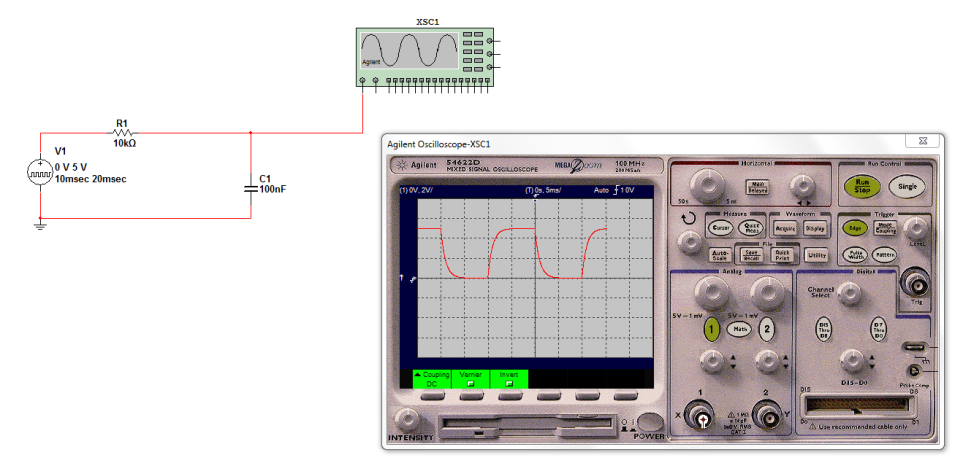
\includegraphics[height=5cm]{P_Fig/figur1.png}
  \caption{Simulering af 1. ordens lavpasfilter}
  \label{1.orden}
 \end{center}
\end{figure}

\begin{figure}[h]
 \begin{center}
  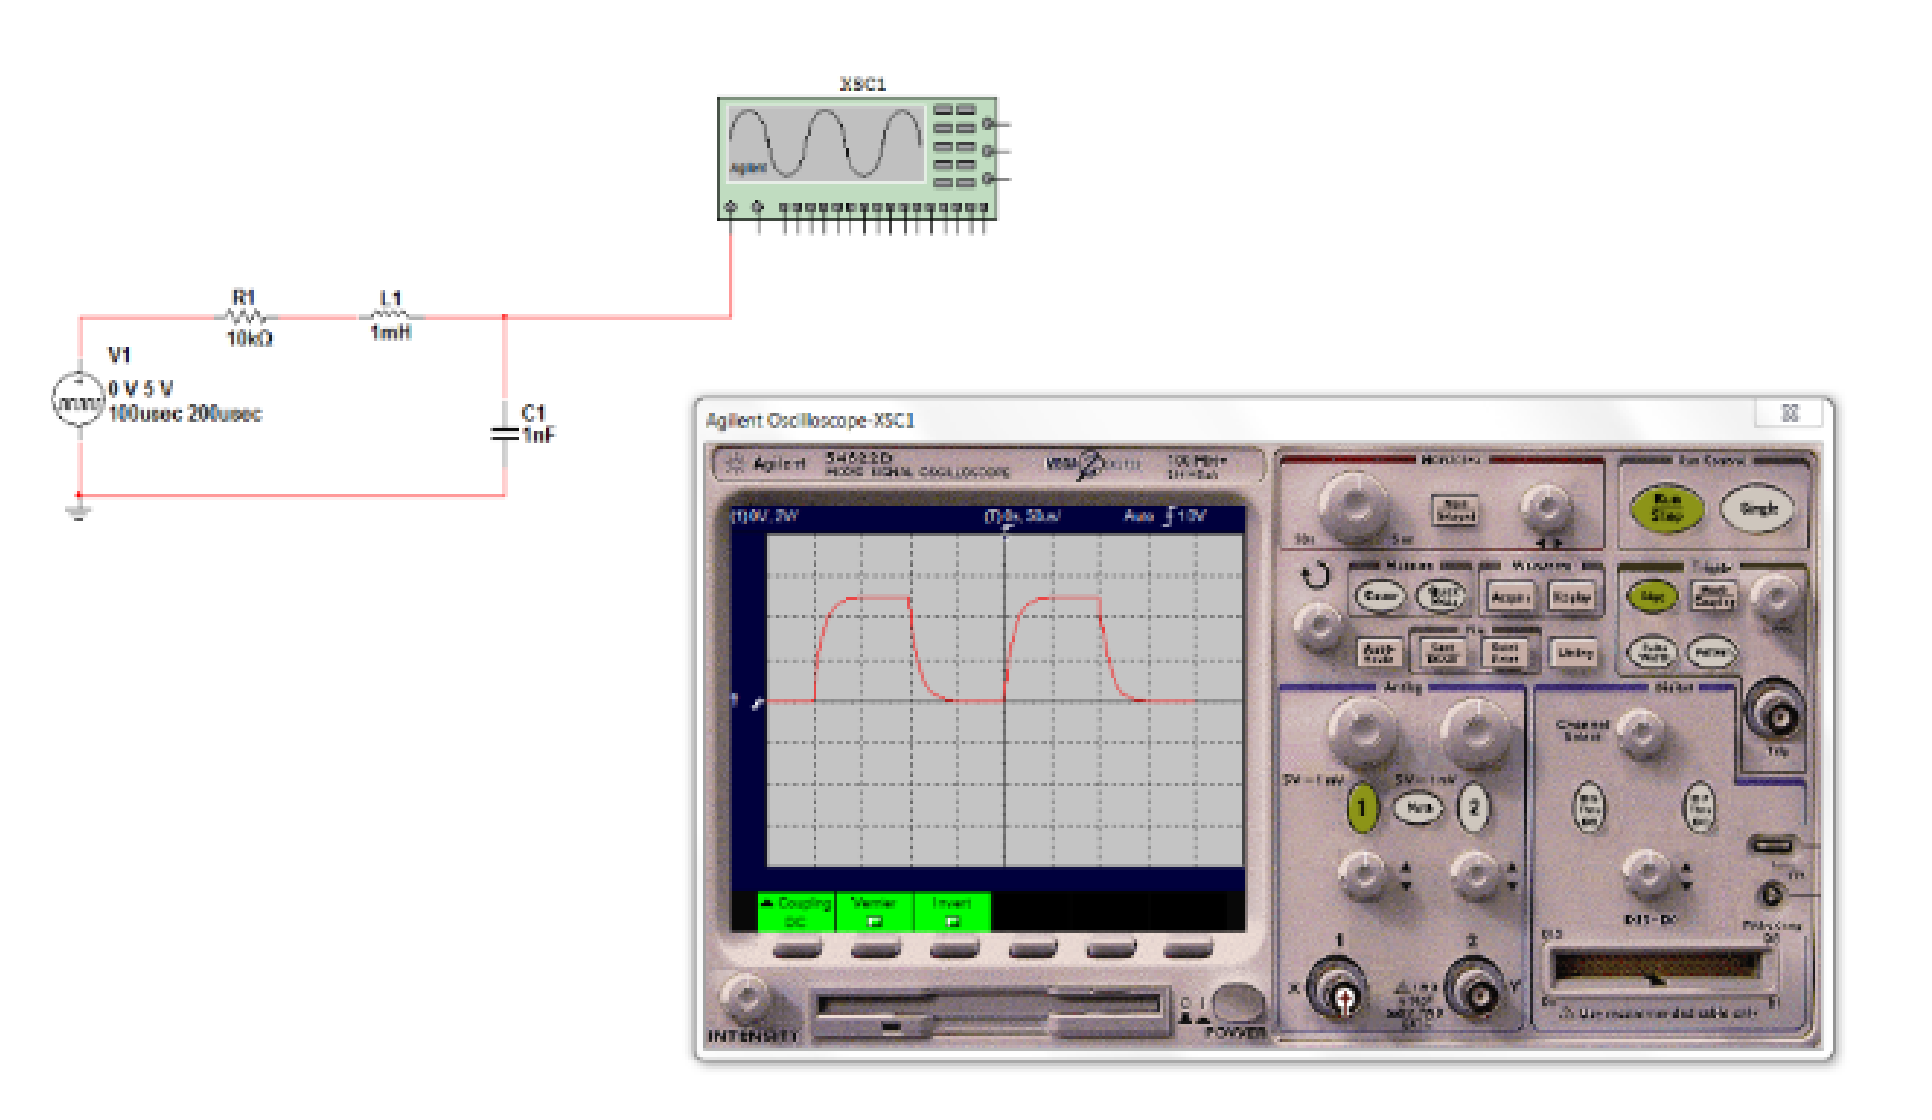
\includegraphics[height=5cm]{P_Fig/figur12_2orden}
  \caption{Simulering af 2.ordens lavpasfilter}
  \label{2orden}
 \end{center}
\end{figure}

\subsubsection{Simulering af 10 k$\Omega$ }
Tidskonstanten($\tau$) bestemmes ved at beregne:

\begin{center}
$V_{max} \cdot 0.63 = V_{\tau}$
\end{center}

Herefter måles tidsforskellen fra $t_0 $ til $t_{\tau}$

$V_{max}$ er ud fra figur \ref{10k.50Hz.tau} målt til 4.97 V
\\ 
$4.97 \ V \cdot 0.63 = 3.131 V$

Tidsforskellen fra $t_0 \ V$ til $V_{\tau}$ måles via figur \ref{10k.50Hz.tau} til 1.01 ms ($\tau$ = 1.01 ms)


\begin{figure}[h]
 \begin{center}
  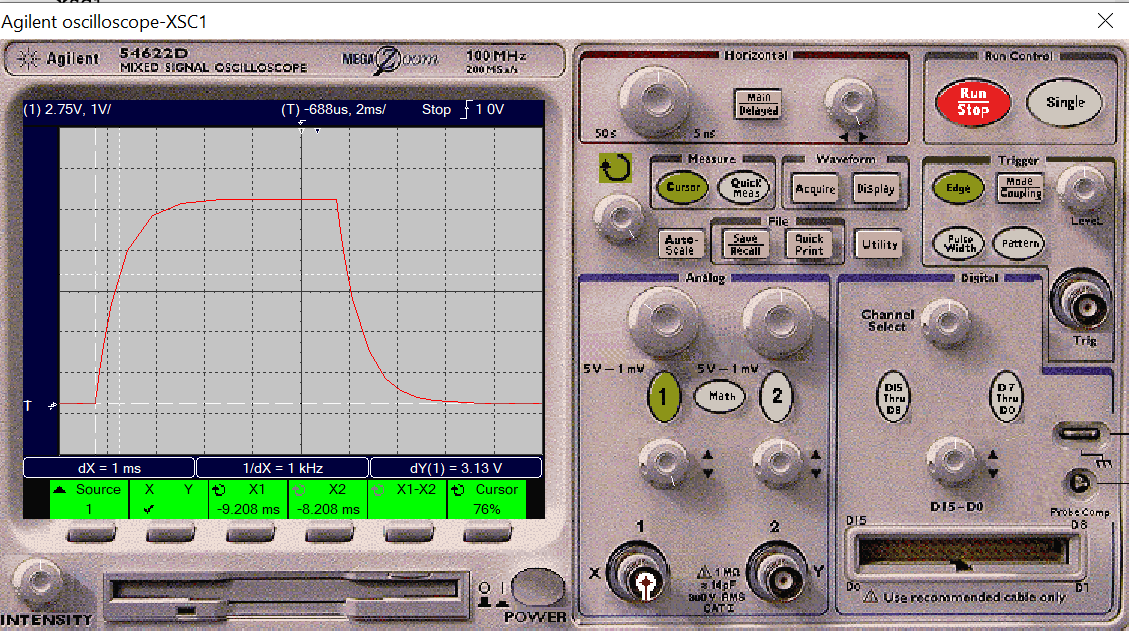
\includegraphics[height=5cm]{P_Fig/figur3_10k_50Hz_tau.png}
  \caption{måling af $\tau$}
  \label{10k.50Hz.tau}
 \end{center}
\end{figure}

Stigetiden bestemmes ved formlen:
\begin{center}
$t_{90} - t_{10} = stigetid$
\end{center}

Ud fra målinger af figur \ref{10k.50Hz.stigetid}
er stigetiden blevet beregnet til

\begin{center}
$t_{10} = 4.97 V \cdot 0.1 = 0.497 V$
\\
$t_{90} = 4.97 V \cdot 0.9 = 4.473 V$
\end{center}

Tidsforskellen mellem $t_{90}$ og $t_{10}$ måles via figur \ref{10k.50Hz.stigetid} til 2.08 ms

\begin{figure}[h]
 \begin{center}
  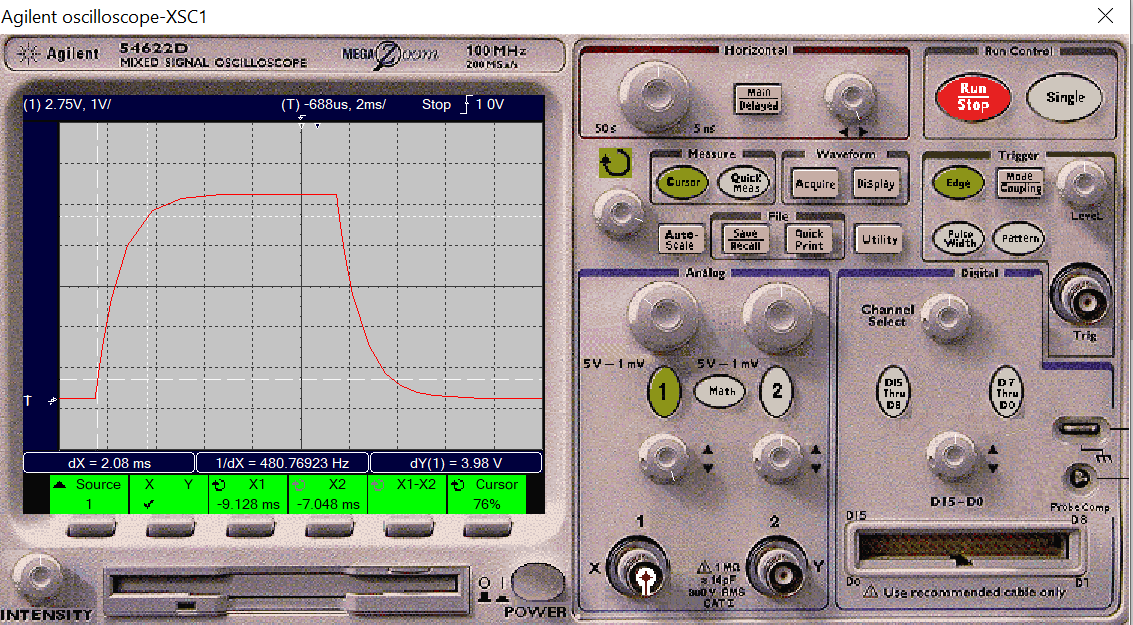
\includegraphics[height=5cm]{P_Fig/figur4_10k_50Hz_stigetid.png}
  \caption{stigetid}
  \label{10k.50Hz.stigetid}
 \end{center}
\end{figure}

Maksimal spænding bestemmes ved formlen:
\begin{center}
$V_{max} - V_{min}$ = Maksimal spænding
\end{center}

Afstanden mellem $V_{max}$ og $V_{min}$ måles via figur \ref{10k.50Hz.min.max} til 4.97 V

\begin{figure}[h]
 \begin{center}
  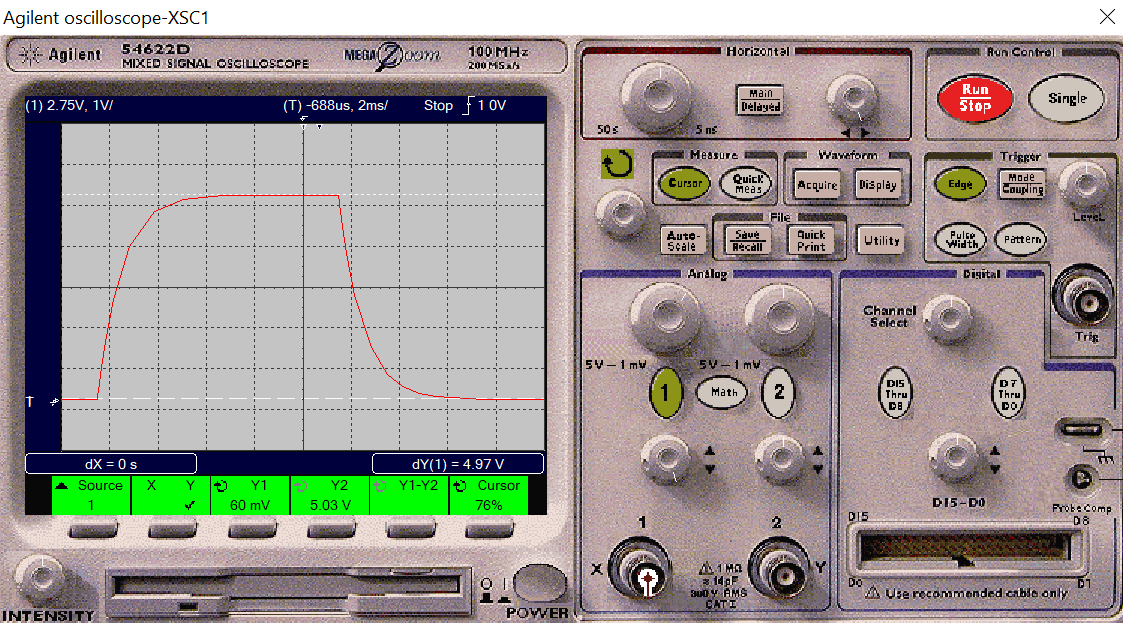
\includegraphics[height=5cm]{P_Fig/figur2_10k_50Hz_min_max.png}
  \caption{Maksimal spænding}
  \label{10k.50Hz.min.max}
 \end{center}
\end{figure}

\newpage
\subsubsection{Simulering af 100 k$\Omega$ }
Tidskonstanten($\tau$) bestemmes ved at beregne:

\begin{center}
$V_{max} \cdot 0.63 = V_{\tau}$
\end{center}

Herefter måles tidsforskellen fra $t_0$ til $t_{\tau}$

$V_{max}$ er ud fra figur \ref{100k_5Hz_tau} målt til 4.96 V
\\
$4.96 \ V \cdot 0.63 = 3.125 V$

Tidsforskellen fra $t_0$ til $t_{\tau}$ måles via figur \ref{100k_5Hz_tau} til 10.04 ms ($\tau$ = 10.04 ms)

\begin{figure}[h]
 \begin{center}
  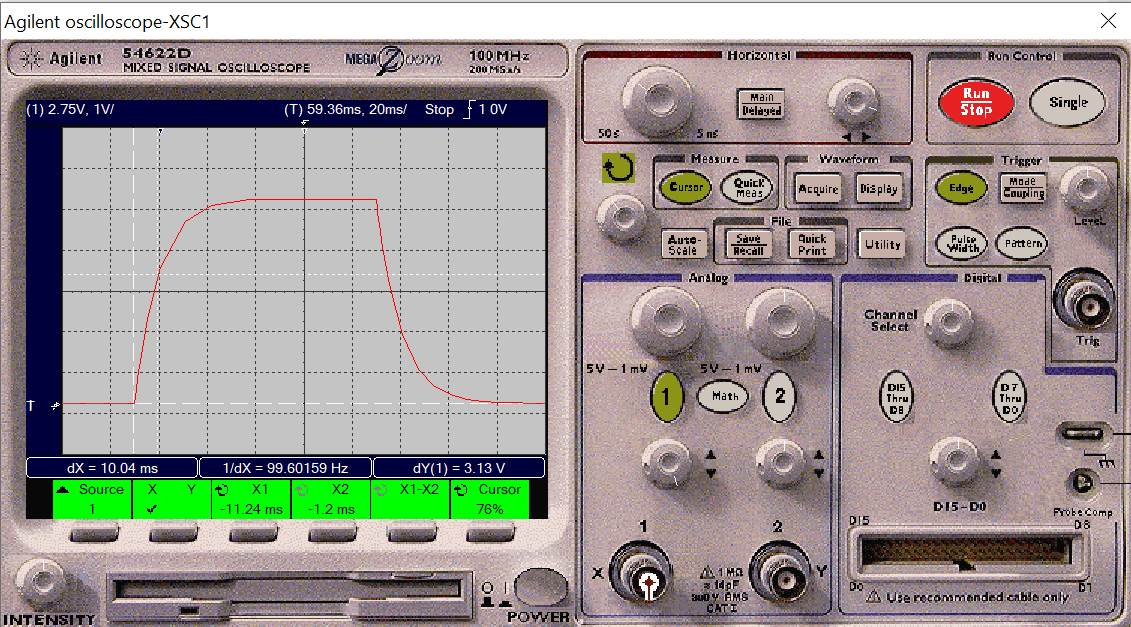
\includegraphics[height=5cm]{P_Fig/figur6_100k_5Hz_tau.png}
  \caption{måling af $\tau$}
  \label{100k_5Hz_tau}
 \end{center}
\end{figure}

\newpage

Stigetiden bestemmes ved formlen:
\begin{center}
$t_{90} - t_{10} = stigetid$
\end{center}

Ud fra målinger af figur \ref{100k.5Hz.stigetid}
er stigetiden blevet beregnet til

\begin{center}
$t_{10} = 4.96 V \cdot 0.1 = 0.496 V$
\\
$t_{90} = 4.96 V \cdot 0.9 = 4.464 V$
\end{center}

Tidsforskellen mellem $t_{90}$ og $t_{10}$ måles via figur\ref{100k.5Hz.stigetid} til 19.72 ms

\begin{figure}[h]
 \begin{center}
  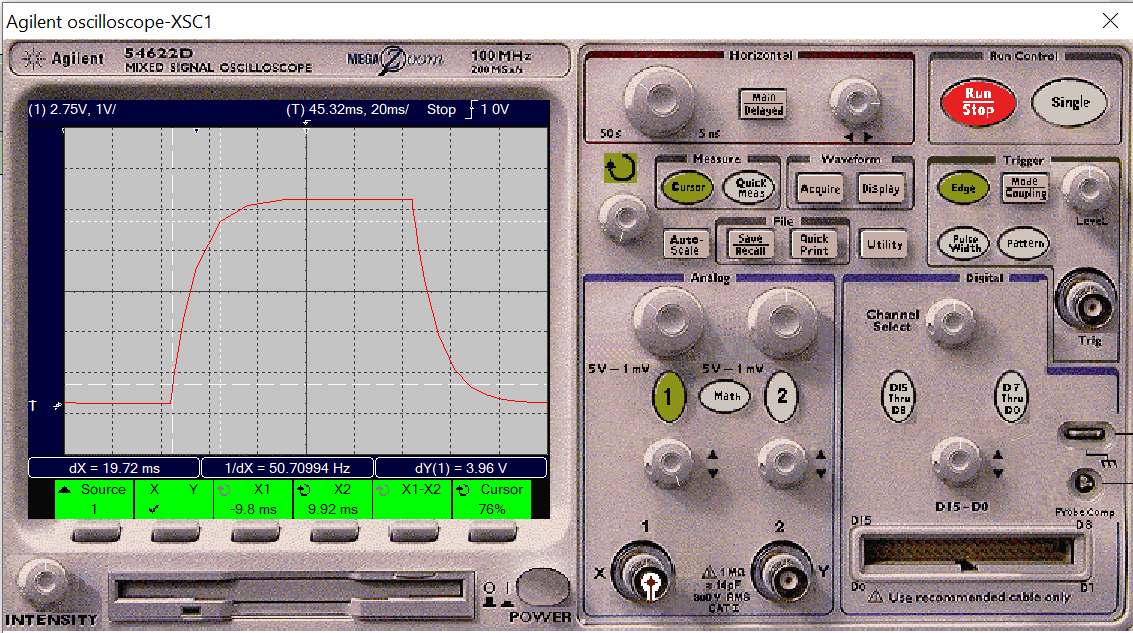
\includegraphics[height=5cm]{P_Fig/figur7_100k_5Hz_stigetid.png}
  \caption{stigetid}
  \label{100k.5Hz.stigetid}
 \end{center}
\end{figure}

Maksimal spænding bestemmes ved formlen:
\begin{center}
$V_{max} - V_{min}$ = Maksimal spænding
\end{center}


Afstanden mellem $V_{max}$ og $V_{min}$ måles via figur \ref{100k.5Hz.min.max} til 4.96 V

\begin{figure}[h]
 \begin{center}
  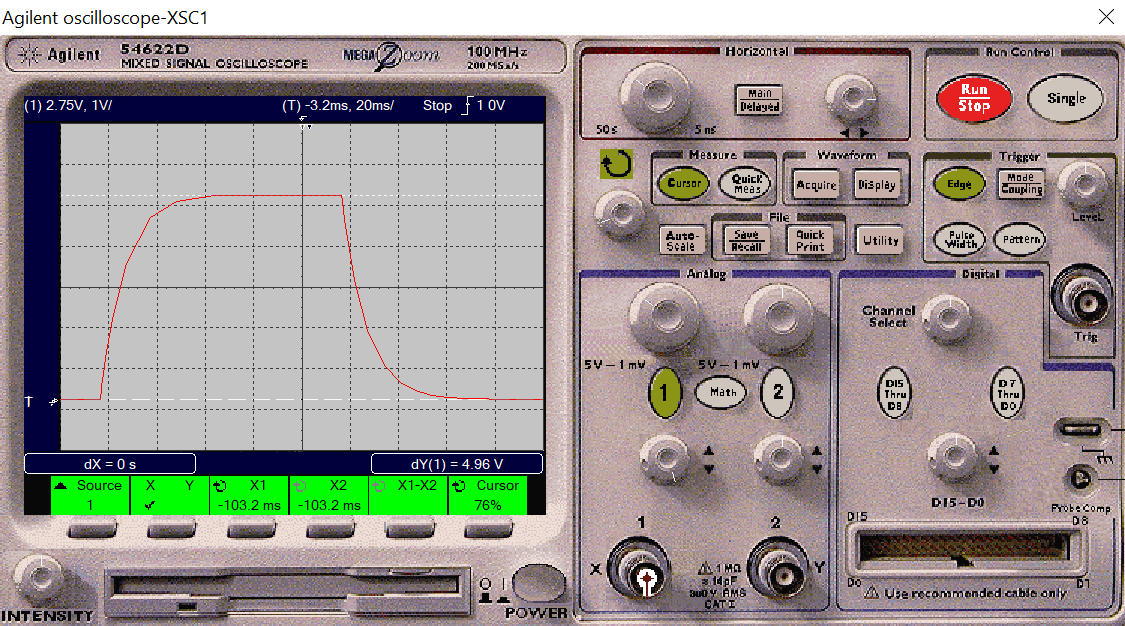
\includegraphics[height=5cm]{P_Fig/figur5_100k_5Hz_min_max.png}
  \caption{Maksimal spænding}
  \label{100k.5Hz.min.max}
 \end{center}
\end{figure}
